\section{Resultados}
% Deben incluir los resultados de los experimentos, utilizando el formato mas
% adecuado para su presentacion. Deberan especicar claramente a que
% experiencia corresponde cada resultado. No se incluiran aqu corridas de
% maquina. Algo fundamental en su aprendizaje en la materia es la presentacion
% de resultados de forma clara y concisa para el lector

% Se incluira aqu un analisis de los resultados obtenidos en la seccion
% anterior (se analizara su validez, coherencia, etc.). Deben analizarse como
% materianimo los lostems pedidos en el enunciado. No es aceptable decir que
% \los resultados fueron los esperados", sin hacer clara referencia a la
% teoremasa a la cual se ajustan. Ademas, se deben mencionar los resul- tados
% interesantes y los casos \patologicos" encontrados.

En esta sección compararemos las diferentes variantes propuestas en este
trabajo. El objeto de este es calcular la inversa de la raíz cuadrada de un
número $\alpha$, por lo que las métricas que nos interesan para decidir entre
variantes es cuánto tarda cada una de las variantes en producir el resultado
esperado y cuán bueno es este.

Dado que una de nuestras premisas es que la magnitud del número incial es
desconocida, analizaremos cada variante para una gran variación de magnitud en
los $\alpha$.

Al igual que en los experimentos de ajustes de parámetros el criterio de parada
elegido para las siguientes pruebas es el de la diferencia relativa. De esta
forma nos aseguramos un error pequeño en relación con la magnitud de cada
$\alpha$. Por ende, compararemos las variantes sólo para resultados ``buenos''.

Por otro lado, utilizaremos cada método ajustando los parámetros en base al
análsis previo visto en la Sección~\ref{sec:ajuste_parametros}.

\subsubsection{Iteraciones}

\begin{figure}[!htbp]
  \begin{center}
    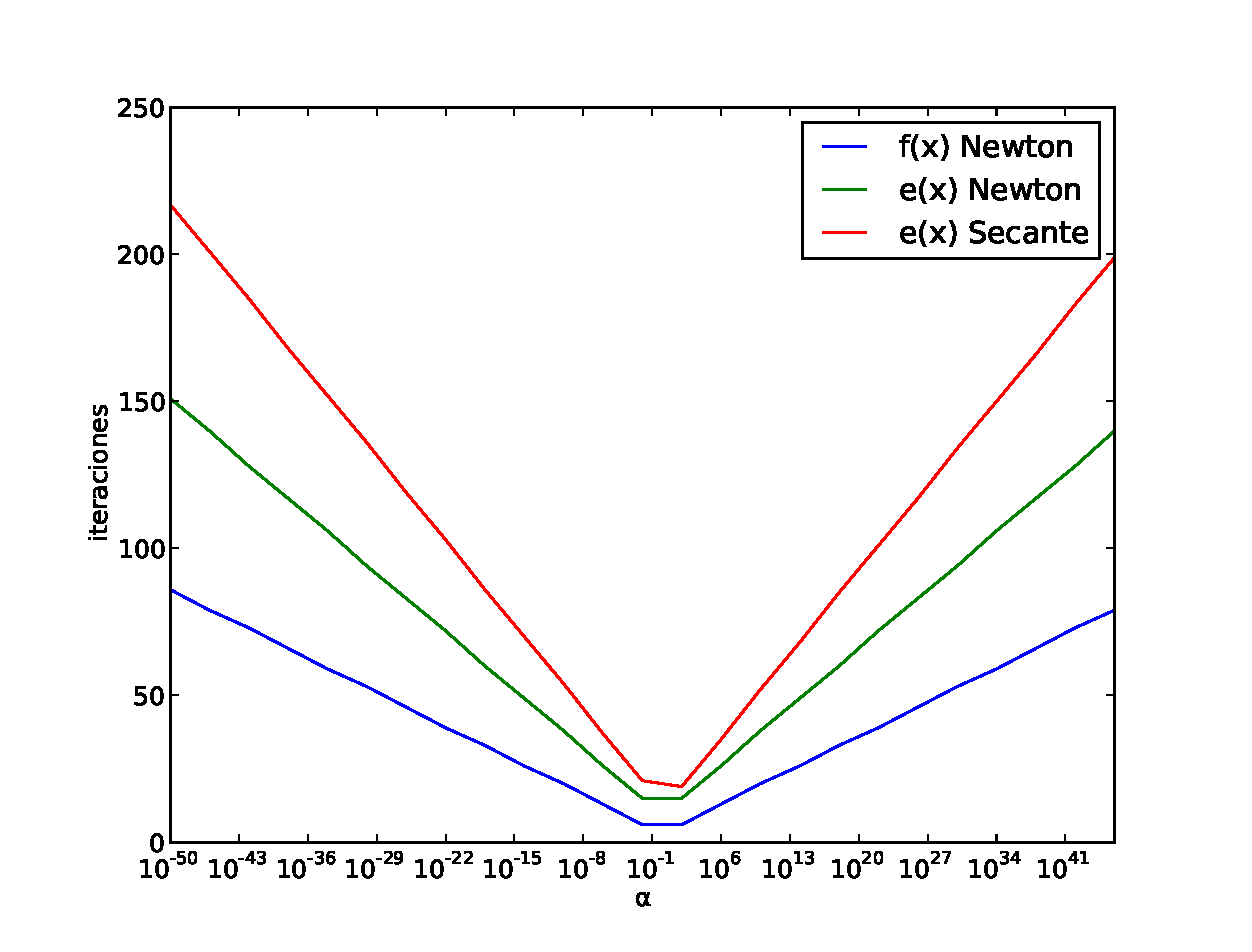
\includegraphics[scale=0.5]{graficos/new/comparacion_iteraciones.eps}
    \caption{\label{fig:comparacion_iteraciones} Cantidad de iteraciones en función de $\alpha$.}
  \end{center}
\end{figure}

Una primer métrica que nos interesa analizar es la cantidad de iteraciones
necesarias para obtener el resultado para diferentes $\alpha$.  En la
Figura~\ref{fig:comparacion_iteraciones} podemos observar esta métrica.

Se puede ver claramente que los $\alpha \simeq 1$ se encuentran beneficiados
con una menor cantidad de iteraciones necesarias. Esto concuerda con nuestro
ajuste de parámetros $x_0$ y $x_1$ ya que decidimos benificiar estos $\alpha$
para equilibrar las iteraciones necesarias para magnitudes pequeñas y grandes
de $\alpha$.

En cuanto a la comparación entre las diferentes variantes observamos, que
$f(x)$ mediante el método de Newton necesita la menor cantidad de iteraciones,
seguido de $e(x)$ mediante el mismo método y por último $e(x)$ mediante el
método de la Secante.

Por último se observa que las pendientes en la cantidad de iteraciones son
similares para magnitudes pequeñas y grandes de $\alpha$.


\subsubsection{Tiempo de Ejecución}

\begin{figure}[!htbp]
  \begin{center}
    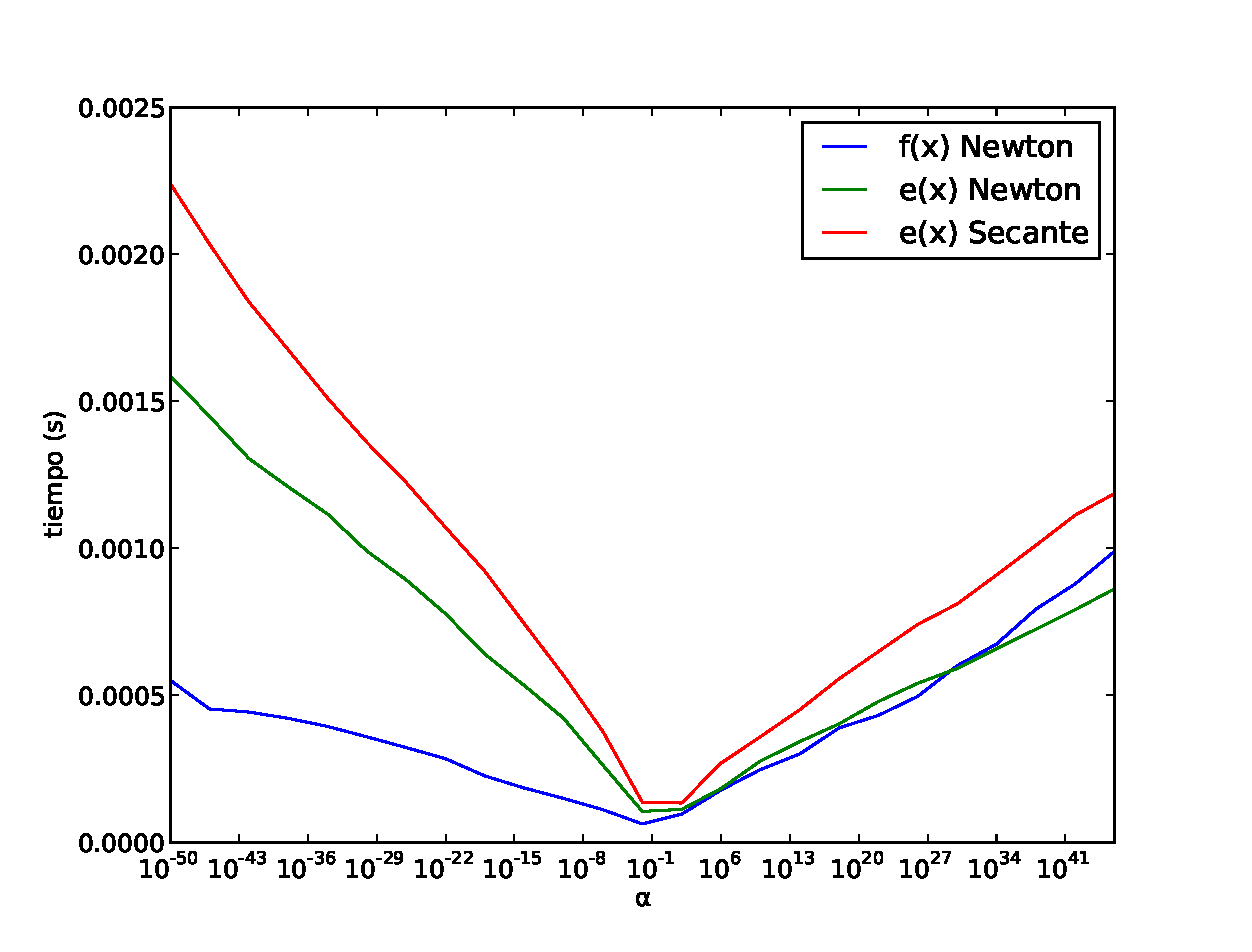
\includegraphics[scale=0.5]{graficos/new/comparacion_tiempos.eps}
    \caption{\label{fig:comparacion_tiempos} Tiempo necesario para llegar al resultado en función de $\alpha$.}
  \end{center}
\end{figure}

No sólo es importante la cantidad de iteraciones que necesita cada variante
sino también el tiempo real necesario para llegar al resultado. En la
Figura~\ref{fig:comparacion_tiempos} realizamos los mismos experimentos que en
la Figura~\ref{fig:comparacion_iteraciones}, pero midiendo el tiempo medio de
1000 ejecuciones.

Notamos cierta correspondencia entre la cantidad de iteraciones necesarias y el
tiempo de ejecución para cada variante. Sobre todo esto es así para $\alpha <
1$ mientras que para $\alpha > 1$ los tiempos parecen acercarse más alla de la
cantidad de iteraciones necesarias.

Para $\alpha > 1$ las variantes de $e(x)$ parecen necesitar menos tiempo por
iteración, mientras que la variante de $f(x)$ parece necesitar más tiempo por
iteración.

No obstante, se observa que $(f)$ mediante el método de Newton necesita menos
tiempo para llegar al resultado.

\newpage
\section{Discusión y Conclusiones}

\subsection{Elección de función y método}

Los resultados obtenidos parecen concordar con nuestras hipótesis inciales. La
variante estudiada de $f(x)$ mediante el método de Newton ofrece los mejores
resultados tanto en cantidad de iteraciones como tiempo necesario para obtener
el resultado.

No obstante es importante notar que si no se cuenta con la derivada de la
función deseada el método de la Secante ofrece buenos resultados.

Por otro lado, nuestra implementación es naive, con un enfoque analítico y no
se encuentra optimizada por lo que los resultados relativos al tiempo de
ejecución pueden cambiar sustancialmente.

No encontramos justificación para la diferencia de pendientes encontradas en la
Figura~\ref{fig:comparacion_iteraciones}. La cantidad de instrucciones
realizadas para $\alpha$ de diferentes magnitudes que necesitan la misma
cantidad de iteraciones es la misma, por lo que no sabemos a que se debe la
disminución o aumento del tiempo de ejecución por iteración para $\alpha > 1$.

\subsection{Ajuste de parámetros}

Nuestro ajuste de parámetros (ver Sección~\ref{sec:ajuste_parametros}) se basa
en no conocer la magnitud de las entradas. Por esta razón decidimos centrar el
análisis en un amplio rango de magnitudes tratando de equilibrar los resultados
entre magnitudes pequeñas y grandes.

De conocerse la magnitud con la cual se trabajará se pueden modificar los
parámetros inciales para beneficiar el tiempo necesario para la obtención de
los resultados dentro de esa magnitud. Esto se puede realizar en base a los
``corrimientos'' que encontramos ocurren modificando las constantes que
utilizamos para calcular cada $x_0$ y $x_1$.

Incluso si no se conoce la magnitud de entrada, se pueden realizar
``particiones'' de los parámetros de entrada, centrando las magnitudes
beneficiadas en cada partición. Esto provee una heurística donde se pueden
agregar cuantas particiones uno desee mejorando el resultado y manteniendo la
cantidad de iteraciones en un rango acotado a lo largo del dominio de los
$\alpha$.

\subsection{Trabajo futuro}

Proponemos el siguiente trabajo futuro basado en los resultados, conclusiones y
experiencias obtenidas a lo largo del desarrollo de este trabajo:

\begin{itemize}

\item Optimizar la implementación. Actualmente contamos con una implementación
naive que puede ser ampliamente optimizada. Creemos que una fuerte optimización
puede traer cambios en los resultados del tiempo de ejecución, sobre todo en el
caso del método de la Secante.

\item Analizar los cambios de pendiente en el tiempo de ejecución para $\alpha$
mayor y menor que 1. No logramos encontrar a que se debe esto, pero creemos que
puede ser aprovechado para mejorar los resultados obtenidos, haciendo uso del
beneficio para tanto $\alpha$ pequeños como para $\alpha$ grandes.

\item Analizar una buena cantidad y distribución de particiones del dominio de
$\alpha$ ajustando los parámetros inciales en cada partición para obtener
mejores resultados para diversas magnitudes.

\end{itemize}
